\usetikzlibrary{positioning}

\begin{document}

\def\title{Worksheet 2}

\newcommand{\qitem}{\qpart\item}

\renewcommand{\labelenumi}{(\alph{enumi})} % change default enum format to (a)
\renewcommand{\theenumi}{(\alph{enumi})} % fix reference format accordingly.
\renewcommand{\labelenumii}{\roman{enumii}.} % second level labels.
\renewcommand{\theenumii}{\roman{enumii}.}

\maketitle

\vspace{0.5em}

\begin{qunlist}

% {\Large \textbf{Mechanical:}}
\qns{Change of Coordinates}
\qcontributor{Yi Zhao, Son Tran, Naomi Sagan, Taejin Hwang}

Many engineering problems can be difficult to solve in its standard xyz coordinates, but may be much easier in a different coordinate system.
In this problem, we will review the process of \emph{change of basis} between coordinate systems.
Remember that a \emph{change of basis} can be represented by a invertible, square matrix.
\par

Let's first start with an example.
Consider the vector $\vec{u} = [u_1, u_2]^T.$ When we write a vector in this form, implicitly we are representing it with the \emph{standard basis} for $\R^{2}$, $\vec{e_1} = [1, 0]^T$ and $\vec{e_2} = [0, 1]^T.$ 

This means that we can write $\vec{u}$ as a linear combination using standard basis vectors $\vec{u} = u_1\vec{e_1} + u_2\vec{e_2}$.
\par

Now, what if we want to represent $\vec{u}$ as a linear combination of another set of basis vectors, say $\vec{a_1} = [1, 1]^T$ and $\vec{a_2} = [0, -1]^T?$
This means that we need to find scalars $u_{a_1}$ and $u_{a_2}$ such that $\vec{u} = u_{a_1}\vec{a_1} + u_{a_2}\vec{a_2}$.
We can write this equation in matrix form:
\[
  \begin{bmatrix}
    | & | \\
    \vec{a_1} & \vec{a_2} \\
    | & |
  \end{bmatrix}
  \begin{bmatrix} u_{a_1} \\ u_{a_2} \end{bmatrix} = \begin{bmatrix} u_{1} \\ u_{2} \end{bmatrix}
.\]
Thus we can find $u_{a_1}$ and $u_{a_2}$ by solving a system of linear equations as seen in 16A.
\par

\meta{
  You can also explain to students that there must be a unique solution, since the U matrix is invertible.
}


\begin{enumerate}
  % Part(a)
  \qitem Let $\vec{v} = [2,-1]^{T}$. What equation gives the coordinates of $\vec{v}$ in the below basis? 
  Try to express your answer in matrix-vector form. No need to do the full calculation.

  \begin{gather*}
    \vec{x} =
    \begin{bmatrix}
      4 \\
      -2
    \end{bmatrix},
    \vec{y} = \begin{bmatrix}
      -3 \\
      -3
    \end{bmatrix}
  \end{gather*}

  % Part(a) solution
  \sol{

    In general, suppose we are given a vector $\vec{u} \in \R^{n}$ in the standard basis and want to change to a different basis with basis vectors $\vec{a_1}, \cdots, \vec{a_n}$.
    If we denote the vector in the new basis as $\vec{u_a} = \begin{bmatrix} u_{a_1} \\ \vdots \\ u_{a_n} \end{bmatrix}$, we solve the following equation $A\vec{u_a} = \vec{u}$, where A is the matrix $\begin{bmatrix} \vec{a_1} & \cdots & \vec{a_n} \end{bmatrix}$.
    Therefore the change of basis is given by:
    \[
      \vec{u_a} = A^{-1}\vec{u}
    .\]

    $$
    \vec{u_a} =
    \begin{bmatrix}
      4 & -3 \\
      -2 & -3
    \end{bmatrix}^{-1}
    \begin{bmatrix}
      2 \\
      -1
    \end{bmatrix}
    $$
  }

  % Part(b)
  \qitem Let $\vec{v} = [3,3]^{T}$. We are told that $\vec{v}$ is represented in the basis:

  \begin{gather*}
    \vec{x} =
    \begin{bmatrix}
      1 \\
      1
    \end{bmatrix},
    \vec{y} = \begin{bmatrix}
      1 \\
      -1
    \end{bmatrix}
  \end{gather*}
  What equation gives the coordinates of $\vec{v}$ in the standard basis?

  % Part(b) solution
  \sol {
    If we already have a vector $\vec{u_a}$ in the basis $\vec{a_1}, \cdots, \vec{a_n}$, how do we change it back to a vector $\vec{u}$ in the standard basis?
    We can reverse the change of basis transformation, thus $\vec{u} = A\vec{u_a}$.
    \par

    $$
    \vec{u_a} =
    \begin{bmatrix}
      1 & 1 \\
      1 & -1
    \end{bmatrix}
    \begin{bmatrix}
      3 \\
      3
    \end{bmatrix}
    $$
  }

 \end{enumerate}

 Now that we've had some mechanical practice, we'll look more into the input-output relationship of vectors.
 For the remaining parts, we'll refer to $[\vec{x}]_S$ or $\vec{x}$ as a vector using standard basis coordinates, and $[\vec{x}]_\beta$ as a vector using $\beta$ basis coordinates.

% Part(c)
 \begin{enumerate}[resume]
  \qitem Let $[\vec{x}]_\beta$ be a vector in $\beta$ coordinates, and $V$ be a change of coordinates matrix from $S \to \beta.$ \\
  How can we represent $\vec{x}$ in terms of $[\vec{x}]_\beta$ and $V?$

  \sol {
    We are given a matrix $V$ that converts standard coordinates to $\beta$ coordinates. 
    This means that $V^{-1}$ will be a matrix that converts $\beta$ coordinates to standard coordinates.
    Therefore, in order to get $\vec{x},$ we multiply $V^{-1}$ with $[\vec{x}]_\beta:$
    $V^{-1} \cdot [\vec{x}]_\beta = [\vec{x}]_S = \vec{x}.$
  }

  % Part(d)
  \qitem Now let $B$ be a linear operator in $\beta$ coordinates. This means that it will take in a vector $[\vec{x}]_\beta$ as an input and output $[\vec{y}]_\beta.$ Given a vector $\vec{x}$ in standard coordinates, why can't we multiply $B \vec{x}$ to get the output $\vec{y}$ in standard coordinates?

  \sol{
    The transformation $B$ "lives" in a different world. It can only accept vectors in $\beta$ coordinates as inputs. 
    Therefore, in order to solve this, we must convert $\vec{x}$ into $\beta$ coordinates.
  }

  % Part(e)
  \qitem Using our $V$ matrix given above, as the change of coordinates matrix from $S \to \beta,$ how can we describe the linear operator $B$ in standard coordinates, that is if $\vec{y} = A \vec{x},$ what is $A$ in the standard basis?

  \sol {
    There will be two main issues we need to address in this question. First off, we need a $\beta$ coordinate input. Secondly, the output of the $B$ is in $\beta$ coordinates, and we will need to convert that back to standard coordinates. 

    Therefore, we take the following steps.

    1. Let's first make our input into $B$ in $\beta$ coordinates. 
    $$\text{Let } \vec{v} = V \vec{x}.$$
    2. Now if we input $\vec{v}$ we will get some output:
    $$\vec{w} = B \vec{v}.$$
    3. However, $\vec{w}$ is in $\beta$ coordinates, so we must convert back to standard coordinates using $V^{-1}.$
    $$\vec{y} = V^{-1} \vec{w}$$
    4. Cascading all of our matrix multiplications, we end up with:
    $$\vec{y} = V^{-1} B V \vec{x}.$$
    Therefore, we can see that $A = V^{-1} B V.$

    The following can also be represented in this state diagram: 

    Note that when cascading transformations, we apply them to the \textbf{left} of the existing transformation.

    \begin{figure}[H]
      \centering
      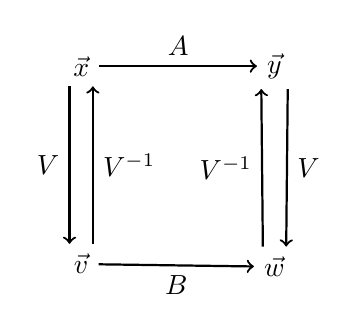
\begin{tikzpicture}[node distance = 2cm, thick]%
        \node (1) {$\vec{x}$};
        \node (2) [right=of 1] {$\vec{y}$};
        \node (3) [below=of 2] {$\vec{w}$};
        \node (4) [below=of 1] {$\vec{v}$};
        \draw[->] (1) -- node [midway,above] {$A$} (2);
        \draw[->] (1.240) -- node [midway,left]{$V$} (4.120);
        \draw[->] (4.60) -- node [midway,right]{$V^{-1}$} (1.300);
        \draw[->] (2.300) -- node [midway,right]{$V$} (3.60);
        \draw[->] (3.120) -- node [midway,left]{$V^{-1}$} (2.240);
        \draw[->] (4) -- node [midway,below] {$B$} (3);
      \end{tikzpicture}%
    \end{figure}
  }
  % % Part(c) solution
  % \sol{
  %   Start by writing $\vec{x_1}$ in terms of $\vec{z_1}$:
  %   $$ \vec{x_1} = V \vec{z_1} $$
  %   Then, apply the transformation $A$ to $\vec{x_1}$, substituting $V \vec{z_1}$ for $\vec{x_1}$:
  %   $$ \vec{x_2} = A V \vec{x_1} $$
  %   Finally, left-multiply both sides by $V^{-1}$ to change $\vec{x_2}$ to the eigenbasis:
  %   $$ \vec{z_2} = V^{-1} \vec{x_2} = V^{-1} A V \vec{z_1} $$

  %   $$A' = V^{-1} A V =
  %   \begin{bmatrix}
  %     1 & 1 \\
  %     -2 & 1
  %   \end{bmatrix}^{-1}
  %   \begin{bmatrix}
  %     3 & -1 \\
  %     -2 & 4
  %   \end{bmatrix}
  %   \begin{bmatrix}
  %     1 & 1 \\
  %     -2 & 1
  %   \end{bmatrix}
  %   $$

  %   $A'$ represents the transformation $A$ in the eigenbasis of $A$, so we know that $A'$ is the diagonal matrix:
  %   $$ A' =
  %   \begin{bmatrix}
  %     \lambda_1 & 0 \\
  %     0 & \lambda_2
  %   \end{bmatrix} =
  %   \begin{bmatrix}
  %     5 & 0 \\
  %     0 & 2
  %   \end{bmatrix} $$

  %   In general, suppose we have a linear transformation $T$ represented by a $n \times n$ matrix that transforms $\vec{u} \in \R^{n}$ to $\vec{v} \in \R^{n}$:
  %   \[
  %     \vec{v} = T\vec{u}
  %   .\]
  %   Suppose we have a basis vectors $\vec{a_1}, \cdots, \vec{a_n} \in \R^{n}$, and the vectors $\vec{u}, \vec{v}$ above are represented in this basis:
  %   \[
  %     \begin{aligned}
  %       \vec{u_a} &= u_{a_1}\vec{a_1} + \cdots + u_{a_n}\vec{a_n} \\
  %       \vec{v_a} &= v_{a_1}\vec{a_1} + \cdots + v_{a_n}\vec{a_n}.
  %     \end{aligned}
  %   \]
  %   Thus we have
  %   \[
  %     \begin{aligned}
  %       T\vec{u}          &= \vec{v} \\
  %       TA\vec{u_a}       &= A\vec{v_a} \\
  %       A^{-1}TA\vec{u_a} &= \vec{v_a}.
  %     \end{aligned}
  %   \]
  %   By pattern matching, we see that if we set $T_a = A^{-1}TA$, we get the relationship $T_a\vec{u_a} = \vec{v_a}$ in the new basis.
  %   The correspondences stated above are all represented in the following diagram:
  %   % \begin{figure}[H]
  %   %   \centering
  %   %   \includegraphics[scale=0.1]{\bank/statespace/figures/change_of_basis.jpg}
  %   % \end{figure}
\end{enumerate}

\newpage
% {\Large \textbf{Mechanical:}}
\qns{An Introduction to Systems}

\meta{You may want to write out the differential equation as:
$$\ddt{}{t} \vec{x}(t) = \ddt{}{t} \begin{bmatrix} x_1 \\ \vdots \\ x_n \end{bmatrix} = \begin{bmatrix} f_1(x_1, .., x_n) \\ \vdots \\ f_n(x_1, .., x_n) \end{bmatrix}$$
}

In the next couple of problem sets, we will be examining systems. 
Many physical systems such as the motion of a car, can be modeled using a system.
Often times, when we are describing a system, we will have a \textbf{state variable $\vec{x},$}
that will often be a multivariable function. 

For a given system, we can often write a differential equation describing its change over time as
\begin{align}
\ddt{}{t}\vec{x}(t) = A \vec{x}(t) + \vec{b}
\end{align}

This differential equation is referred to as a \textbf{vector differential equation} 
and is a generalization of single variable differential equations to the multivariate case.
In this context, $A$ is a $n \times n$ matrix, and $\vec{b}$ is a scalar vector in $\mathbb{R}^n.$

Given the following system:
\begin{align*}
    \ddt{}{t}x_{1}(t) &= 3 x_{1}(t) - 2 x_{2}(t) \\
    \ddt{}{t}x_{2}(t) &= - x_{1}(t) + 5 x_{2}(t)
\end{align*}

With initial conditions $x_{1}(0) = 2, \ x_{2}(0) = 3,$

\begin{enumerate}
    \qitem What is an appropriate state vector for this system?

    \sol{
        We have to variables $x_1$ and $x_2$ therefore we define our state vector as:
        $$\vec{x} = \begin{bmatrix} x_{1} \\ x_{2} \end{bmatrix}$$
    }

    \qitem What is the initial condition of this system?

    \sol{
        We have the individual initial conditions for $x_1$ and $x_2$ but we must also a define an initial condition for our state vector.
        $$\vec{x}(0) = \begin{bmatrix} x_{1}(0) \\ x_{2}(0) \end{bmatrix} = \begin{bmatrix} 2 \\ 3 \end{bmatrix} $$
    }

    \qitem Write out the system of differential equations as a vector differential equation.
    
    \sol{
        $$\ddt{}{t}\vec{x}(t) = \begin{bmatrix} 3 & -2 \\ -1 & 5 \end{bmatrix} \begin{bmatrix} x_{1}(t) \\ x_{2}(t) \end{bmatrix} 
        = \begin{bmatrix} 3 & -2 \\ -1 & 5 \end{bmatrix} \vec{x}(t) $$
    }
\end{enumerate}

% \qitem Explain why the system 
%     \begin{align*}
%         \ddt{x}{t} &= ax + by \\
%         \ddt{y}{t} &= cx + dy
%     \end{align*}
%     can be equivalently formulated as
%     \[
%         \ddt{}{t} \begin{bmatrix} x \\ y \end{bmatrix} = \begin{bmatrix} a & b \\ c & d \end{bmatrix} \begin{bmatrix} x \\ y \end{bmatrix}
%     \]


% \qitem Given the following system:
%     \begin{align*}
%         \ddt{x}{t} &= x \\
%         \ddt{y}{t} &= y
%     \end{align*}

%     With initial conditions $x(0) = x_0, \ y(0) = y_0,$

%     \begin{enumerate}
%         \qitem What is an appropriate state vector for this system?
%         \qitem What is the initial condition of this system?
%         \qitem Convert this system into its State-space representation.
%         \qitem How can you solve for $x(t)$ and $y(t)?$
%     \end{enumerate}

\newpage
% Authors: Tony Li
% Emails: songli@berkeley.edu

\qns{Thevenin's and Norton's Equivalent Circuit}

In this set, we will review two useful theorems that you might have learned in previous physics classes.
\textbf{Thevenin's Theorem} states that we can replace entire network by an equivalent circuit that contains only an independent voltage source in series with an impedance (resistor) such that the current-voltage relationship at the load is unchanged.
\begin{figure}[H]
  \centering
  \begin{circuitikz}[american]
    \draw (6, 0) node[ocirc, label=right:\(B\)]{} to[short] (4, 0) to[R] (2, 0) to[V] (0, 0) to[short] (0, 4) to[V] (2, 4) to[I, invert] (4, 4) to[short] (6, 4) node[ocirc, label=right:\(A\)]{};
    \draw (2, 0) to[R] (2, 4);
    \draw (4, 0) to[I] (4, 2) to[R] (4, 4);

    \path[draw=black, thick, -Triangle] (7, 2) -- (9, 2);

    \draw (12, 1) node[ocirc, label=right:\(B\)]{} to[short] (10, 1) to[V, invert] (10, 3) to[R] (12, 3) node[ocirc, label=right:\(A\)]{};
  \end{circuitikz}
  \caption{Thevenin's Equivalent Circuit}
  \label{fig:thevenin-example}
\end{figure}
As shown above, we have a linear electrical network, containing only voltage sources, curretn sources, resistors, and two terminals A and B.
The circuit can be always transformed to an equivalent circuit with only one voltage source, one resistor, and two terminals A and B.
By using this theorem, we can largely simplfy the circuit.
A more easier way to understand this is that we can use a black box to include everything connecting to two terminals, and then replace the black box with a voltage source and a resistor in series.

\textbf{Norton's Thereom} is identical to Thevenin's Theorem except that the equivalent circuit is an independent current source in parallel with an impedance (resistor).
Therefore, the Norton equivalent circuit is a source transformation of the Thevenin equivalent circuit.
\begin{figure}[H]
  \centering
  \begin{circuitikz}[american]
    \draw (6, 0) node[ocirc, label=right:\(B\)]{} to[short] (4, 0) to[R] (2, 0) to[V] (0, 0) to[short] (0, 4) to[V] (2, 4) to[I, invert] (4, 4) to[short] (6, 4) node[ocirc, label=right:\(A\)]{};
    \draw (2, 0) to[R] (2, 4);
    \draw (4, 0) to[I] (4, 2) to[R] (4, 4);

    \path[draw=black, thick, -Triangle] (7, 2) -- (9, 2);

    \draw (12, 1) node[ocirc, label=right:\(B\)]{} to[short] (10, 1) to[I] (10, 3) to[short] (12, 3) node[ocirc, label=right:\(A\)]{};
    \draw (11, 1) to[R] (11, 3);
  \end{circuitikz}
  \caption{Norton's Equivalent Circuit}
  \label{fig:norton-example}
\end{figure}
Quite similar to Thevenin's theorem, we can replace a linear electrical network with a current source and a resistor in parallel.Note that, the power source can be non-constant, which means that we could have an AC circuit.
As a result, we need to use impedances at a given frequency substituting the resistances.

First, let's assume that the voltage source is ideal and does not have any internal resistance.
In a non-ideal case, we need to add one more resistor beside the voltage source to represent the internal resistance of the voltage source.
However, for an ideal current source, it has infinite internal resistance.
Then use KVL, KCL, and Ohm's Law to find out the resistance and voltage in the Thevenin's equivalent circuit.
Similar procedure also applies to the Norton's equivalent circuit.

For the following problems, we will first try to obtain the Thevenin's equivalent circuit of the following circuit.
\begin{figure}[H]
  \centering
  \begin{circuitikz}[american]
    \draw (7, 0) node[ocirc, label=right:\(B\)]{} to[short] (0, 0) node[ground]{} to[V, l2=\(V_s\) and \SI{25}{\volt}, invert] (0, 2) to[R, l2=\(R_1\) and \SI{5}{\ohm}, l2 valign=b] (3, 2) to[short] (5, 2) to[R, l2=\(R_3\) and \SI{4}{\ohm}, l2 valign=b] (7, 2) node[ocirc, label=right:\(A\)]{};
    \draw (3, 0) to[R, l2=\(R_2\) and \SI{20}{\ohm}] (3, 2);
    \draw (5, 0) to[I, l2=\(I_s\) and \SI{3}{\ampere}] (5, 2);
  \end{circuitikz}
  \caption{Circuit to examine}
  \label{fig:q3}
\end{figure}

\begin{enumerate}
  % Part(a)
  \qitem
   First, we need to create an imaginary wire connecting to terminal \(A\) and \(B\), and also a terminal \(C\).
   \begin{figure}[H]
    \centering
    \begin{circuitikz}[american]
      \draw (7, 0)  to[short] (0, 0) node[ground]{} to[V, l2=\(V_s\) and \SI{25}{\volt}, invert] (0, 2) to[R, l2=\(R_1\) and \SI{5}{\ohm}, i=\(I_{R_1}\), l2 valign=b] (3, 2) node[ocirc, label=above:\(C\)]{} to[short] (5, 2) to[R, l2=\(R_3\) and \SI{4}{\ohm}, i<^=\(I_{R_3}\), l2 valign=b] (7, 2);
      \draw (3, 0) to[R, l2=\(R_2\) and \SI{20}{\ohm}, i_=\(I_{R_2}\)] (3, 2);
      \draw (5, 0) to[I, l2=\(I_s\) and \SI{3}{\ampere}] (5, 2);
      \draw (7, 2) node[ocirc, label=right:\(A\)]{} to[short, i=\(I_{AB}\)] (7, 0) node[ocirc, label=right:\(B\)]{};
    \end{circuitikz}
    \caption{Determining short-circuit current}
    \label{fig:q3a}
  \end{figure}
  Denote the voltage at terminal \(C\) as $V_c$.
  What are the magnitudes of the currents $I_{R_1}$, $I_{R_2}$, $I_{R_3}$?
  By using KCL, can you derive an equation including all four currents?

  \meta {
    Please ask students why it is important to use KCL?
    How do we know that by using KCL we can get the value of $V_c$?
    $I_{R_2}$ is negative because the direction of the current $I_{R_2}$ is from ground to terminal C.
    It does not mean that the magnitude of $I_{R_2}$ is negative.
    In KCL, whether the current is negative or postive is determined by its direction.
  }

  \sol{
    We create the following node voltage equations by KCL:
    \begin{align*}
      I_{R_1} &= \frac{V_s - V_c}{R_1} \\
      I_{R_2} &= -\frac{V_c}{R_2} \\
      I_{R_3} &= -\frac{V_c}{R_3} \\
      I_s + I_{R_1} + I_{R_2} + I_{R_3} &= 0 \\
    \end{align*}
    Because we have created a wire from terminal \(A\) to \(B\), terminal \(A\) is grounded now.
    Plugging in, we get
    \begin{align*}
      I_s + \frac{V_s - V_c}{R_1} - \frac{V_c}{R_2} - \frac{V_c}{R_3} &= 0 \\
      I_s + \frac{V_s}{R_1} - V_c \left(\frac
      {1}{R_1} + \frac{1}{R_2} + \frac{1}{R_3}\right) &= 0 \\
      \implies V_c = \frac{I_s + \frac{V_s}{R_1}}{\frac
      {1}{R_1} + \frac{1}{R_2} + \frac{1}{R_3}} &= \SI{16}{\volt}
    \end{align*}
  }

  % Part(b)
  \qitem After establishing the equation, you should be able to find out $V_C$.
  Based on the value of $V_C$, what is the magnitude of $I_{ab}$?
  $I_{ab}$ is called \textbf{short-circuit current}, it is the current that actually flow from A to B if you connect two terminals in the equivalent circuit.

  \sol {
    Apply KCL at terminal A, and we get
    \begin{equation*}
      I_{ab} = -I_{R_3} = \frac{V_c}{R_3} = \SI{4}{\ampere}
    \end{equation*}
  }

  %part c
  \qitem Then, suppose that there is \textbf{no such imaginary wire across A and B}.
  Let's focus on finding the value of the \textbf{Thevenin Equivalent Resistance} $R_{th}$.
  To calculate the Thevenin equivalent resistance, remove all power sources from the original circuit.
  The voltage sources are short-circuited and current sources are opened.
  What is $R_{th}$, the total resistance between terminal A and B in the remaining circuit? \\
  \emph{Hint:} The remaining circuit now only has three resistors. $R_1$ and $R_2$ are now in parallel and $R_3$ is in series with $R_1$ and $R_2$.
  \begin{figure}[H]
    \centering
    \begin{circuitikz}
      \draw (7, 0) node[ocirc, label=right:\(B\)]{} to[short] (0, 0) node[ground]{} to[short] (0, 2) to[R, l2=\(R_1\) and \SI{5}{\ohm}, l2 valign=b] (3, 2) to[short] (5, 2) to[R, l2=\(R_3\) and \SI{4}{\ohm}, l2 valign=b] (7, 2) node[ocirc, label=right:\(A\)]{};
      \draw (3, 0) to[R, l2=\(R_2\) and \SI{20}{\ohm}] (3, 2);
      % \draw (5, 0) to[I, l2=\(I_s\) and \SI{3}{\ampere}] (5, 2);
    \end{circuitikz}
    \caption{Circuit with nulled sources}
    \label{fig:q3b}
  \end{figure}
  \meta {
    We need the imaginary wire to calculate the short-circuit current $I_{ab}$ in Thevenin's equivalent circuit.
    Now, deleting that wire helps us to find out the total resistance between A and B $R_{th}$.
    Why is the voltage source like a wire and the current source like an open-circuit?
    Because we are using ideal power sources, and the voltage source has no internal resistance and the current source has infinite internal resistance.
  }

  \sol {
    Now the voltage source acts like a wire, and the total resistance between \(A\) and \(B\) is
    \begin{equation*}
      R_{tg} = R_1 \parallel R_2 + R_3 = \frac{R_1 R_2}{R_1 + R_2} + R_3 = \SI{8}{\ohm}
    \end{equation*}
  }

  % Part(d)
  \qitem We are almost done! Now, it's time to draw our Thevenin's equivalent circuit.
  \begin{figure}[H]
    \centering
    \begin{circuitikz}
      \draw (2, 0) node[ocirc, label=right:\(B\)]{} to[short] (0, 0) to[V, l=\(V_{th}\), invert] (0, 2) to[R, l=\(R_{th}\)] (2, 2) node[ocirc, label=right:\(A\)]{};
    \end{circuitikz}
    \caption{Thevenin equivalent circuit for this problem}
    \label{fig:q3d}
  \end{figure}
  What are the values of $V_{th}$ and $R_{th}$? \\
  \emph{Hint:} What law should we use to get $V_{th}$? Remember $I_{ab}$ is the short-circuit current.

  \meta {
    Please explain thoroughly why we need the imaginary current at the first place.
    If we want to get $V_{th}$ in the equivalent circuit, we need to connect two terminals first in the equivalent cicuit, and then apply Ohm's Law.
  }

  \sol{
    $R_{th}$ is just what we have found previously as \SI{8}{\ohm}.
    $V_{th} = I_{ab} \cdot R_{th} = \SI{32}{\volt}$, by Ohm's Law.
  }
  \end{enumerate}

  Now we know how to get a Thevenin's Equivalent Circuit, but how do we get a Norton's Equivalent Circuit?
  In this question we will look at how to use Thevenin's Circuit to get the Norton's Circuit.

  \begin{enumerate}[resume]
  % Part(e)
  \qitem Let's look at the same graph, Figure 3. You have already obtained the value of the short-circuit current $I_{ab}$ and
  the total resistance $R_{th}$ between the terminal A and B. Why don't we just use both of the values to find out $I_{th}$ and $R_{th}$ in the Norton's equivalent circuit shown below?
  \begin{figure}[H]
    \centering
    \begin{circuitikz}
      \draw (2, 0) node[ocirc, label=right:\(B\)]{} to[short] (0, 0) to[I, l=\(I_{th}\)] (0, 2) to[short] (2, 2) node[ocirc, label=right:\(A\)]{};
      \draw (1, 0) to[R, l_=\(R_{th}\)] (1, 2);
    \end{circuitikz}
    \caption{Norton equivalent circuit for this problem}.
    \label{fig:q4e}
  \end{figure}
  \meta {
    Explain that why we can use the same data we got previously. We can still apply Ohm's Law to get $I_{th}$ and $R_{th}$.
  }

  \sol {
    $R_{th}$ in Norton is equal to $R_{th}$ in Thevenin for the same circuit, because if you consider the current source has an open-circuit, $R_{th}$ in Norton is also the total resistance between terminal A and B.
    That is, $R_{th} = \SI{8}{\ohm}$ and $I_{th} = \frac{V_{ab}}{R_{th}} = \SI{4}{\ampere}$.
    Two helpful properties of Thevenin and Norton equivalences:
    \begin{enumerate}
      \item Thevenin resistance and Norton resistance are equal.
      \item Thevenin voltage is equal to the Norton current times the Norton resistance.
      That is, \(V_{th} = I_n \cdot R_{th}\).
    \end{enumerate}
  }

\end{enumerate}

\end{qunlist}

\end{document}
